\subsection{逻辑化简法}
\label{subsec:lab4-logic-minimization}

\paragraph{基本原理}

前面我们通过Hamming距离，为每个不可达点构造一条线性不等式，从而将其排除。

但是这样有一个问题，就是如果不可达点太多，那么需要添加的约束也会非常多

那能不能用一条约束同时排除多个不可达点呢？
\begin{figure}[H]
    \centering
    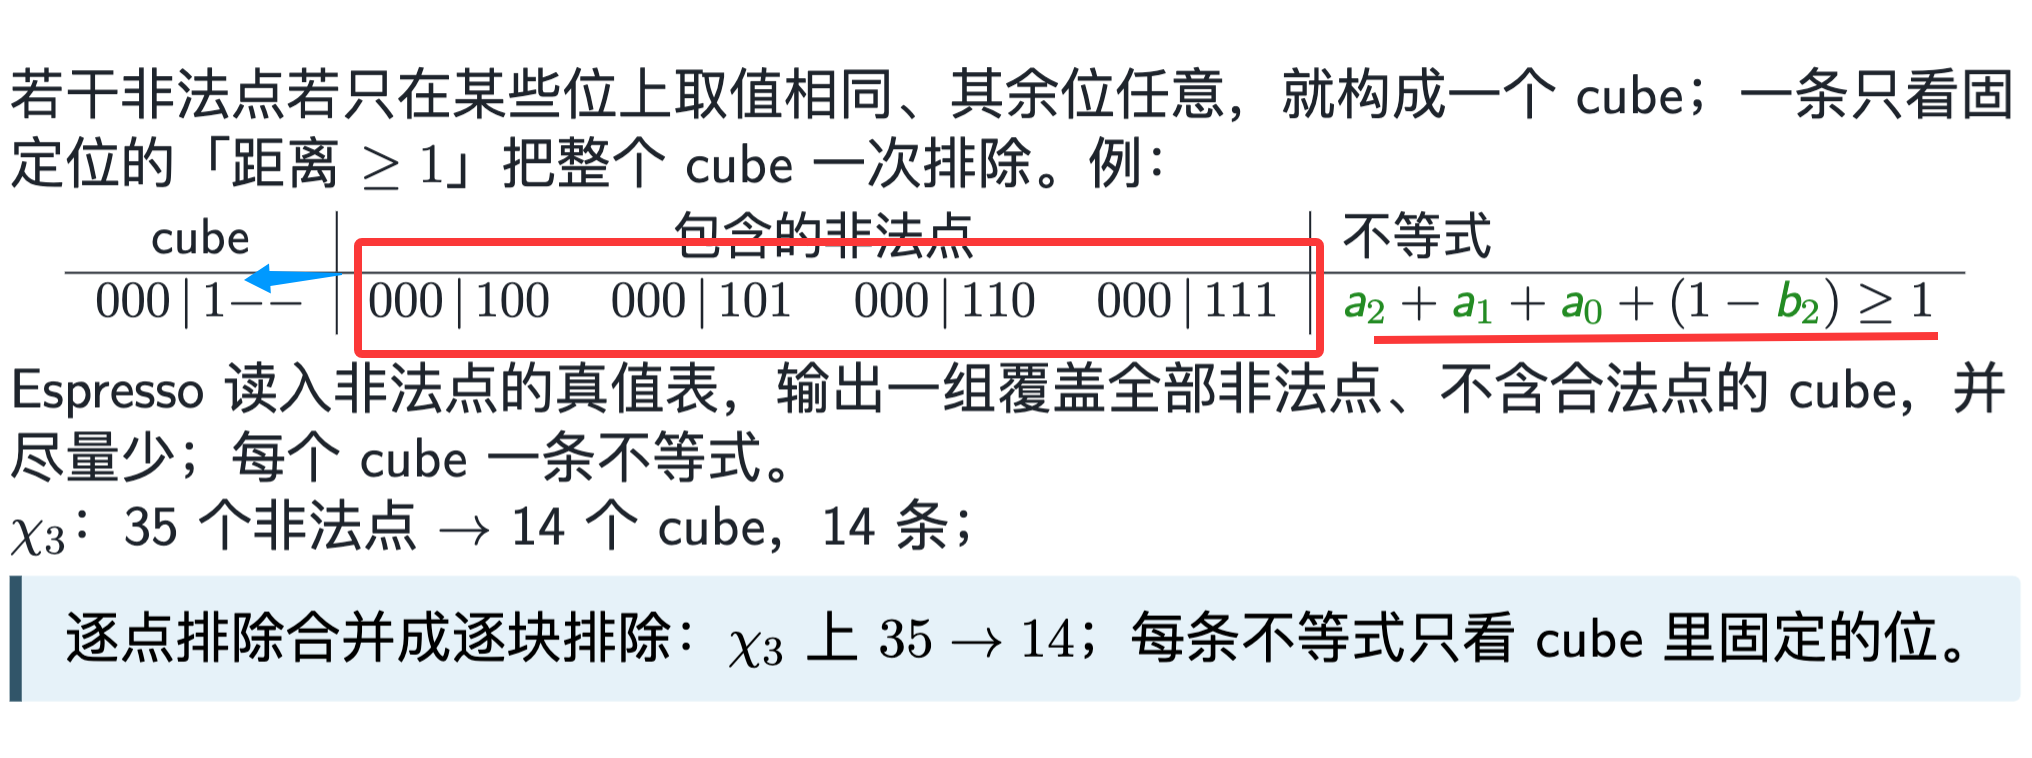
\includegraphics[width=0.8\textwidth]{figures/logic.png}
\end{figure}
就比如课件里这个例子,不可达点的前四位都是0001,那这样我们就可以合并成一个不等式，本来是需要四个的

逻辑化简法将这些点作为布尔函数的取值为$1$的输入，其实就有点像数字逻辑里的卡诺图化简

通过Espresso等工具合并为cube，再对每个cube建立一条排除约束

一条这样的约束可以同时排除该cube覆盖的全部不可达的点


\paragraph{不可达点的布尔表示}


首先，设不可达点集合为
\[
Q=\{0,1\}^{8}\setminus V.
\]

我们定义一个布尔函数
\[
f_{\mathrm{bad}}(x)=
\begin{cases}
1,&x\in Q,\\
0,&x\in V.
\end{cases}
\]

接下来，我们可以把这个函数的真值表交给逻辑化简工具，尝试把多个不可达点合并起来

一般来说，一个cube可以写成
\[
c=(c_1,\ldots,c_8)\in\{0,1,-\}^{8}.
\]

其中$0$和$1$表示对应位置必须取固定值，而$-$表示这一位可以任意取值

为了方便后面构造约束，我们记
\[
I_0(c)=\{j\mid c_j=0\},
\qquad
I_1(c)=\{j\mid c_j=1\}.
\]

那么，一个cube所表示的全部二进制点就是
\[
B(c)=\left\{
x\in\{0,1\}^{8}\;\middle|\;
x_j=0\ (j\in I_0(c)),
\ x_j=1\ (j\in I_1(c))
\right\}.
\]

假设经过逻辑化简后，我们得到了一个cube集合$\mathcal C$，那么我们希望这些cube恰好覆盖所有不可达点，即
\begin{equation}
\bigcup_{c\in\mathcal C}B(c)=Q.
\label{eq:lab4-cube-cover}
\end{equation}

这里要注意，所谓恰好覆盖，不仅要求所有不可达点都包含在这些cube中，还要求不能把任何可达点也包含进去。

讲义使用\texttt{espresso-logic}读取PLA格式的非法点列表：本实验应声明八个输入、一个输出，输入标签按$a_3,a_2,a_1,a_0,b_3,b_2,b_1,b_0$排列，每个非法点的输出标为$1$，未列出的点按对应PLA输入模式解释为输出$0$，不能当作任意取值。读取化简结果时，逐行提取输出为$1$的cube；其中的\texttt{-}表示该位不限，\texttt{.p}字段表示输出的cube数量。无论采用讲义中的\texttt{-Dexact}方式，还是通过其他接口调用Espresso，后续线性化都依赖式\eqref{eq:lab4-cube-cover}所要求的精确覆盖关系。


\paragraph{cube的线性约束}

如果要排除一个cube，只需要保证$x$至少有一个固定坐标与cube不一致即可

至于那些取值为$-$的坐标，就不需要考虑了

对于一个cube $c$，我们可以构造如下约束：
\begin{equation}
\begin{aligned}
\min\quad &0\\
\text{s.t.}\quad
&\sum_{j\in I_0(c)}x_j
+\sum_{j\in I_1(c)}(1-x_j)\ge1,
&&\forall c\in\mathcal C,\\
&x_j\in\{0,1\},
&&j=1,\ldots,8.
\end{aligned}
\label{eq:lab4-cube-model}
\end{equation}

我们也可以将常数项移到右边，得到
\[
\sum_{j\in I_0(c)}x_j-\sum_{j\in I_1(c)}x_j
\ge1-|I_1(c)|.
\]

例如，假设有一个cube
\[
c=0000\,000-.
\]

那么我们只需要构造
\[
x_1+x_2+x_3+x_4+x_5+x_6+x_7\ge1.
\]

这样就同时排除了$0000\,0000$和$0000\,0001$两个点

\paragraph{正确性分析}

对于任意一个cube $c\in\mathcal C$，如果$x\in B(c)$，那么$x$的所有固定坐标都与$c$一致。

也就是说，当$c_j=0$时，有$x_j=0$；当$c_j=1$时，有$x_j=1$。

因此，
\[
\sum_{j\in I_0(c)}x_j
+\sum_{j\in I_1(c)}(1-x_j)=0,
\]
不满足约束条件，所以$x$被排除。

反过来，如果$x\notin B(c)$，那么至少存在一个固定坐标与$c$不同，因此上式左边至少为$1$，满足对应的约束。

这就说明，一条约束恰好可以排除一个cube覆盖的全部二进制点，而不会影响cube之外的点。

接下来考虑所有cube构成的集合$\mathcal C$。

根据前面逻辑化简得到的覆盖关系
\[
\bigcup_{c\in\mathcal C}B(c)=Q,
\]
我们知道，所有cube恰好覆盖全部不可达点。

因此，对于任意可达点$x\in V$，它不属于任何cube覆盖的点集，所以能够满足全部约束，模型不会遗漏合法传播。

反过来，如果$x\notin V$，那么$x\in Q$，根据覆盖关系，必然存在某个cube $c\in\mathcal C$使得$x\in B(c)$，从而违反对应的约束。

因此，所有不可达点都会被排除。

综上，模型的二进制可行解集合恰好为$V$，即
\[
\left\{
x\in\{0,1\}^{8}\;\middle|\;
\sum_{j\in I_0(c)}x_j+
\sum_{j\in I_1(c)}(1-x_j)\ge1,
\ \forall c\in\mathcal C
\right\}=V.
\]

这样，我们就利用逻辑化简，将原来针对每个不可达点的约束，合并成了针对每个cube的约束。

对于差分传播，我们可以对DDT中值为$0$的位置进行化简；对于线性传播，则可以对LAT中值为$0$的位置进行化简。
